\documentclass[tikz, border=5pt]{standalone}
\usepackage{amsmath, pgffor}
\usepackage[x11names]{xcolor}
\usetikzlibrary{calc, positioning}

\begin{document}
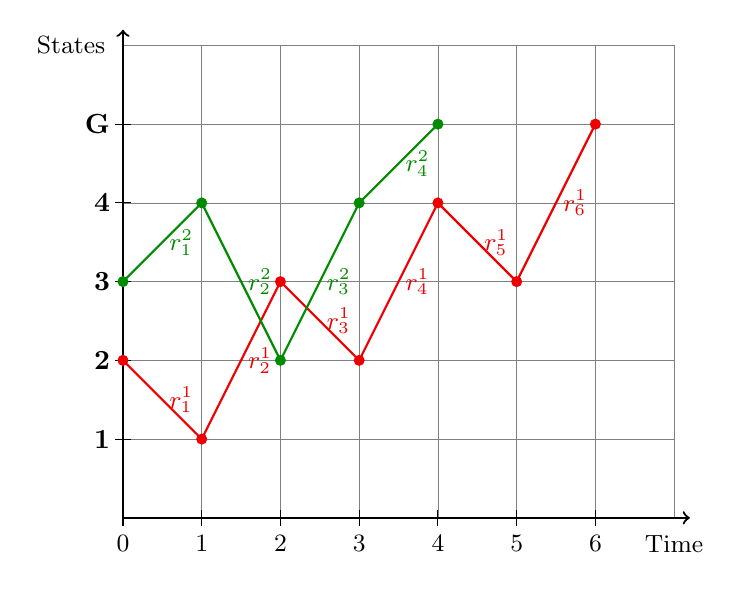
\begin{tikzpicture}

    \NewDocumentCommand{\trajectory}{ m m m }{
        \global\edef\seg{1}
        \global\edef\prevx{-1}
        \global\edef\prevy{-1}
        \foreach \x/\y in {#3} {
                \fill[#2] (\x,\y) circle (2pt);
                \pgfmathparse{\prevx > -1}
                \ifnum \pgfmathresult=1
                    \draw[#2, thick] (\prevx,\prevy) -- (\x,\y);
                    \node at ($(\prevx,\prevy)!0.5!(\x,\y)$) [above=2pt, right=-1pt, #2, font=\small]
                    {\( r^{#1}_{\pgfmathprintnumber[fixed, precision=0]{\seg}} \)};
                    \pgfmathparse{\seg+1} \global\edef\seg{\pgfmathresult}
                \fi
                \global\edef\prevx{\x}
                \global\edef\prevy{\y}
            }
    }

    %% Grid
    \newcommand{\xmax}{7} \newcommand{\ymax}{6}
    \draw[gray, very thin] (0,0) grid (\xmax,\ymax);
    \draw[thick, ->] (0,0) -- (\xmax+0.2,0);
    \node at (\xmax, -0.1) [below] {\small Time};
    \draw[thick, ->] (0,0) -- (0,\ymax+0.2);
    \node at (-0.1, \ymax) [left] {\small States};
    \pgfmathsetmacro{\xend}{\xmax-1}
    \foreach \x in {0,...,\xend}
    \draw (\x,0.1) -- (\x,-0.1) node[below] {\small \( \x \)};
    \pgfmathsetmacro{\yend}{\ymax-2}
    \pgfmathsetmacro{\terminal}{\ymax-1}
    \foreach \y in {1,...,\yend}
    \draw (-0.1,\y) -- (0.1,\y) node[left=4pt] {\( \mathbf \y \)};
    \draw (-0.1,\terminal) -- (0.1,\terminal) node[left=4pt] {\textbf G};

    % Trajectories
    \trajectory{1}{Red2}{0/2, 1/1, 2/3, 3/2, 4/4, 5/3, 6/5}
    \trajectory{2}{Green4}{0/3, 1/4, 2/2, 3/4, 4/5}

\end{tikzpicture}
\end{document}
